\begin{figure}[t]
\begin{center}
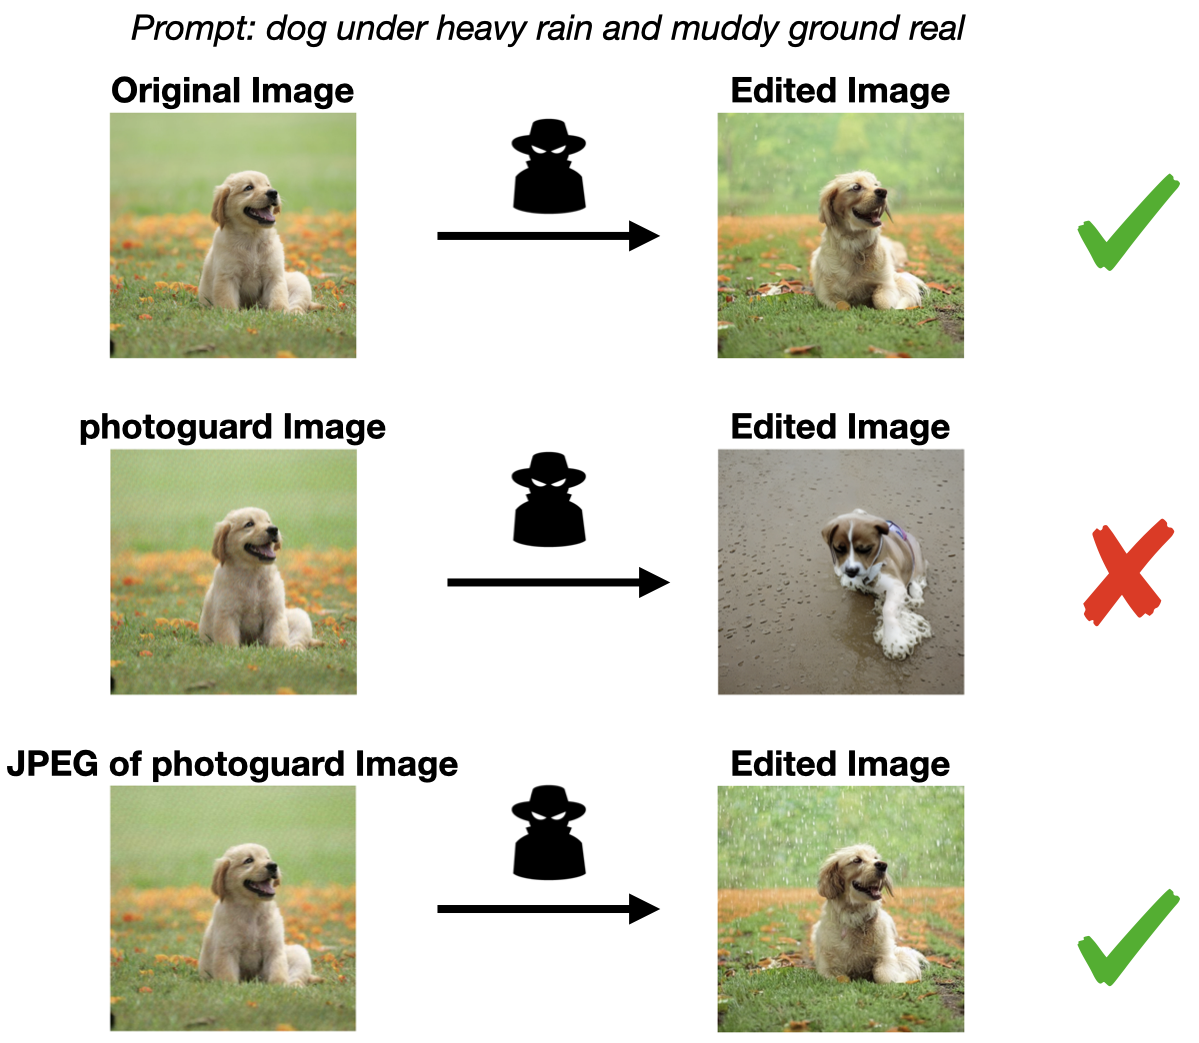
\includegraphics[width=0.7\textwidth]{images/2-overview-figure.001.png}
\end{center}
\caption{\textbf{JPEG compression allows an adversary to modify a protected image found online.} First row: Given a text prompt, an adversary can make desired edits to an input image using a diffusion model. Second row: photoguard (Encoder attack) \citep{salman2023raising} protects the original image before an adversary can access it by adding an imperceptible perturbation. When the adversary edits the photoguard image, they are unable to maintain the original subject. Third row: By JPEG compressing the photoguard image, an adversary can edit the photoguard image while maintaining the original subject and adding key visual features of the text prompt.}
\label{fig:img2img-overview}
\end{figure}